\begin{problem}{Trapping Rain Water}
    Given n non-negative integers representing height of building in one-dimension. Assuming width of each building as 1unit. Compute how much water will be trapped by these building.

    \footnotetext{LC42}
\end{problem}

\begin{solution}[solution summary]
    There are various ways to solve this problem.

    \begin{guide}

        TO-DO: Add images in guide/hint section.

        \item For current building, if you could find what is leftmost building which is just greator than arr[i] and what is rightmost building which is just greator then arr[i]. (i.e previousGreatorElement + nextGreatorElement).
        
        Then, water trapped by arr[i] would be \verb|min(pg,ng)-arr[i]|

        Try to use DP to calculate pgarr and ngarr.

        \item Can you use stack to find pg and ng for arr[i]?
        
        \item Can you try to use two-pointer?
    \end{guide}

\end{solution}

\begin{solution}[Stack | O(n)]
    Lets use stack to solve this problem.

    Recall that, stack can help us find previousGreatorElement and nextGreatorElement in linear time.
    
    If you focus on nge and pge for element arr[i], then you need to first find pgarr[] and ngarr[] then solve your problem.

    But, if you focus on nge and pge \textbf{for element being popped}. Then you know the nge and pge just after the element is being popped.

    \begin{marginfigure}
        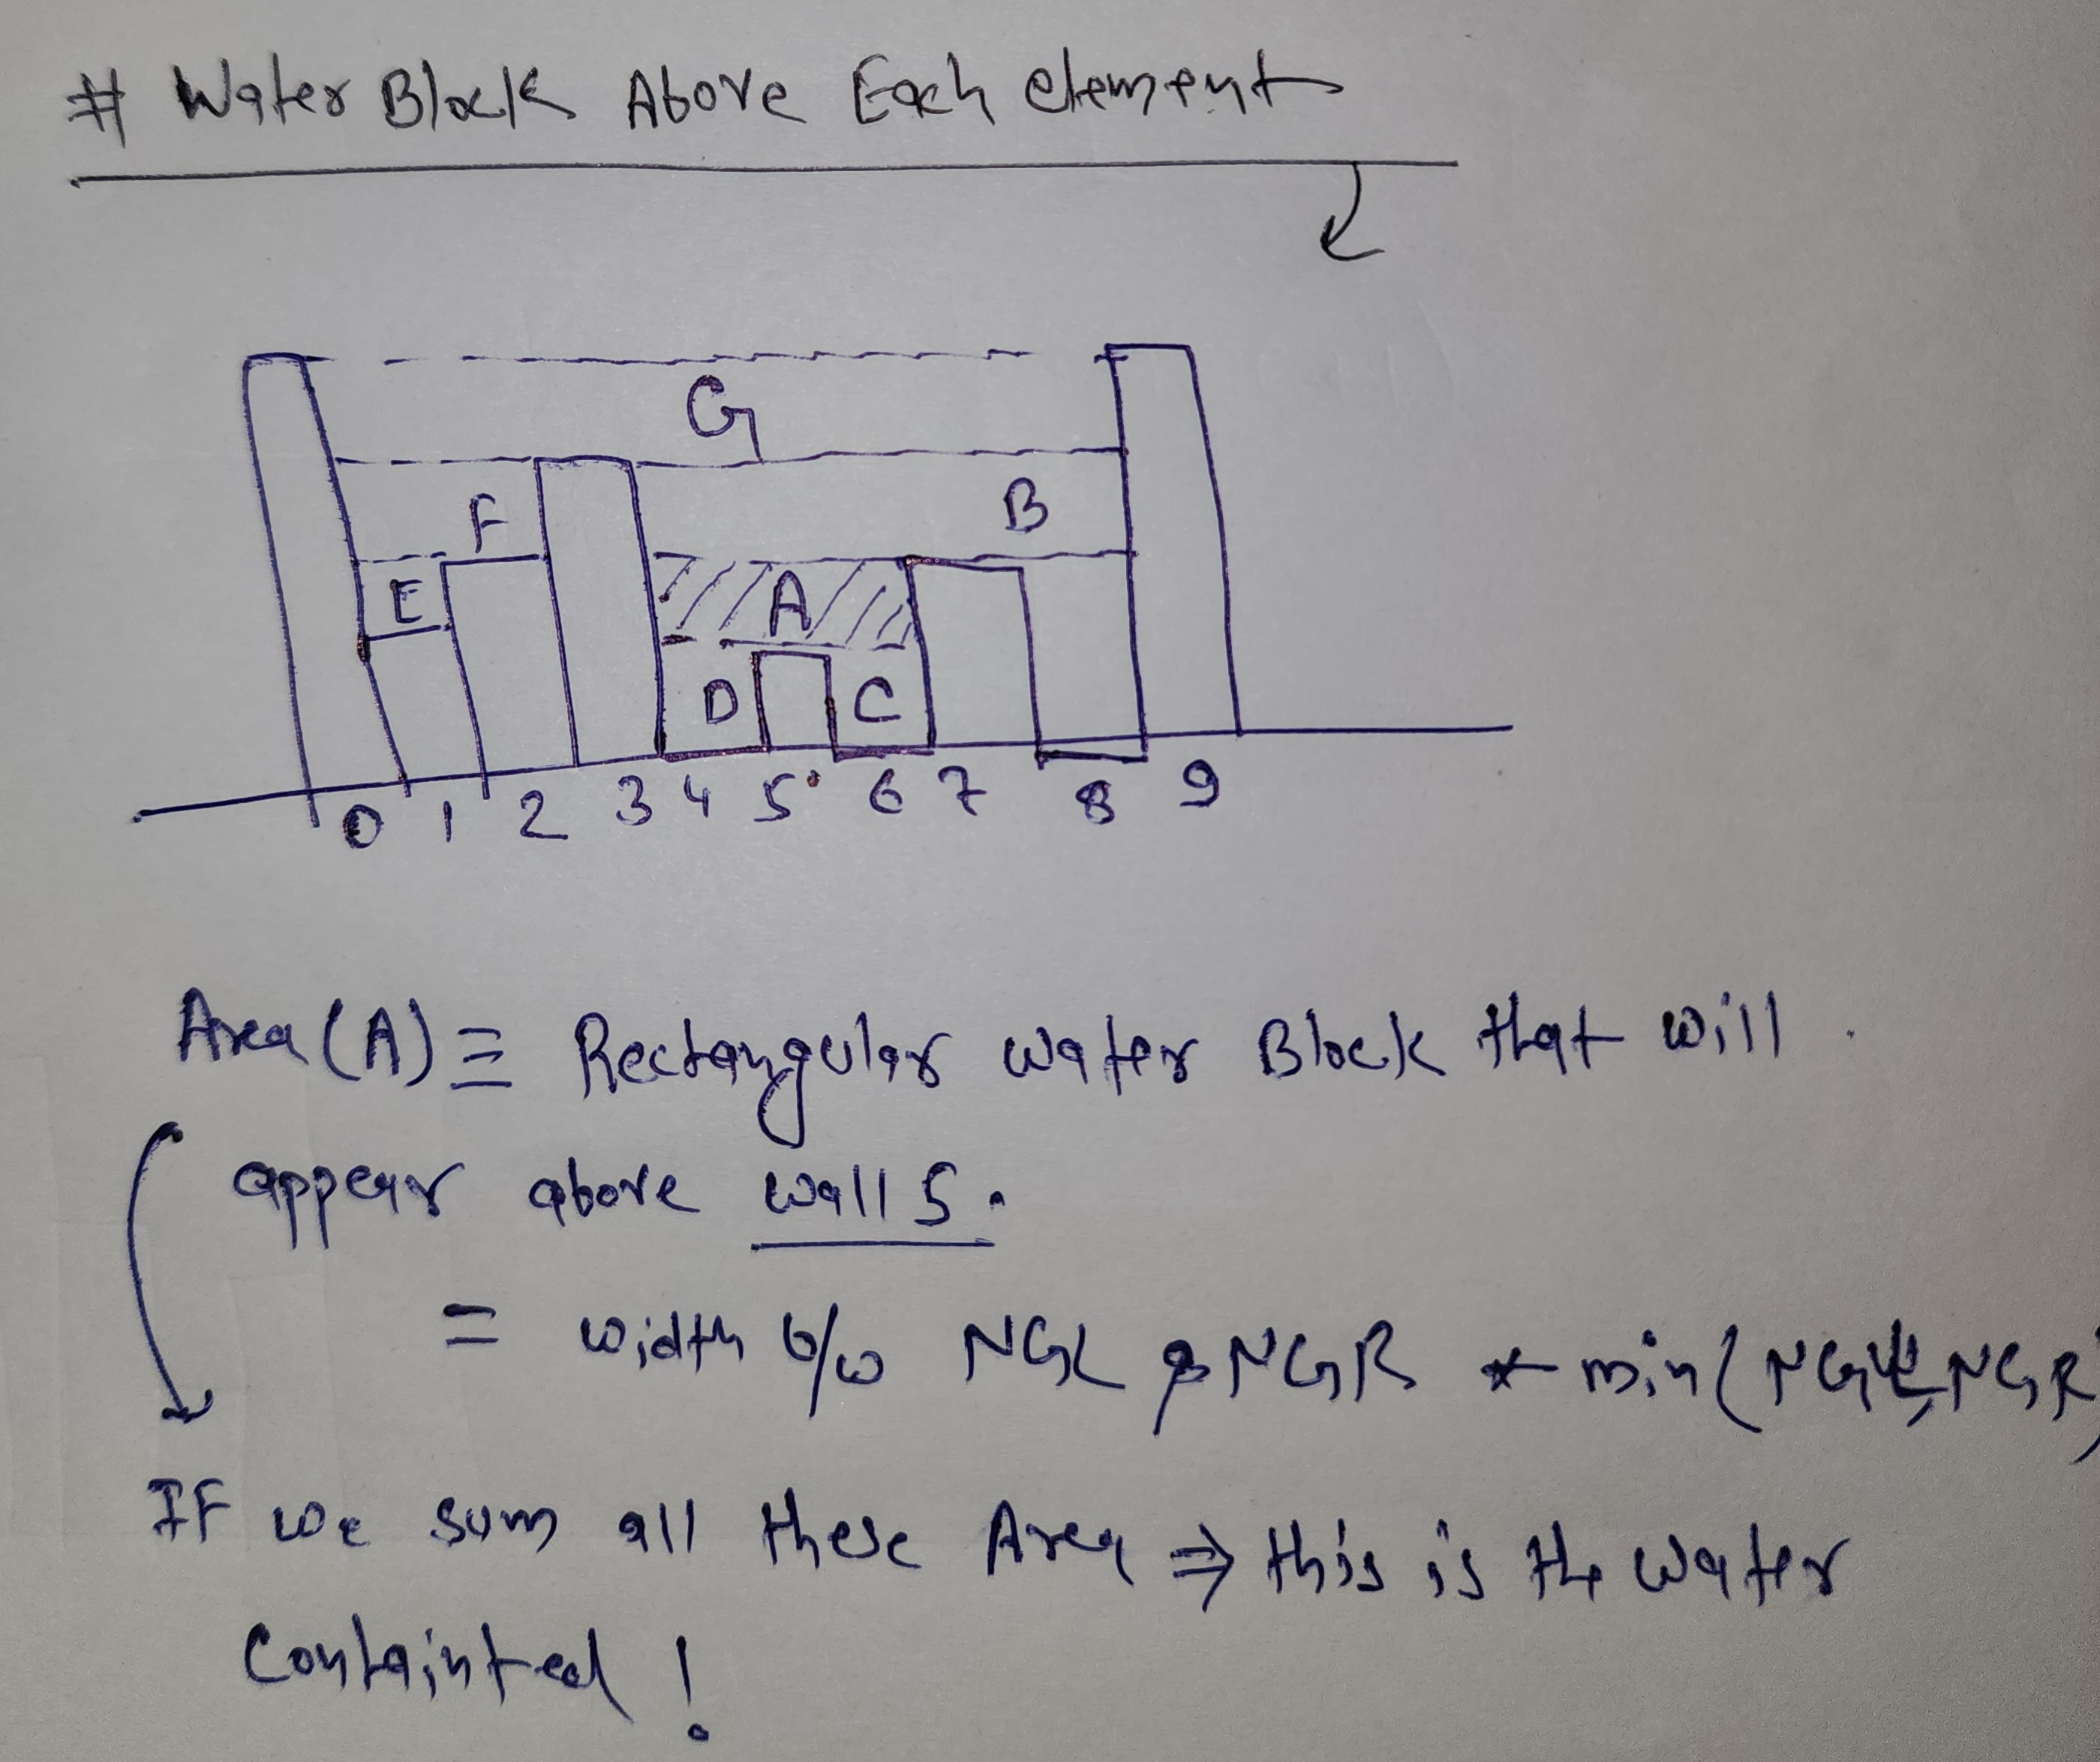
\includegraphics[width=\marginparwidth]{resources/stack-rain-water-harvesting-1.jpg}
    \end{marginfigure}
    \begin{code3}
        int trapStack(vector<int>& arr) 
        {
            vector<int> st;
           
            int sum = 0;
            for(int i=0;i<arr.size();i++)
            {
                while(!st.empty() && arr[tidx]<arr[i])
                {
                    int eidx = tidx; //popped element
                    st.pop_back();
                    
                    if(st.empty() == true)
                        continue;
                    
                    /* for popped stack element*/
                    int pgei = tidx; //previous greator element
                    int ngei = i; //next greator element
     
                    int water = min(arr[pgei],arr[ngei]) - arr[eidx];
                    water = water*(ngei-pgei-1);
                                 
                    sum += water;
                    
        //            printf("%d,%d,%d: %d\n",arr[pgei],arr[eidx],arr[ngei],water);
                }
                
                st.push_back(i);
            }
            
            return sum;
        }
    \end{code3}
\end{solution}

\begin{solution}[DP | O(n)]
    Find lmax[] and rmax[].
    Then water bar trapped above each element be\\
    \verb|min(lmax[i],rmax[i])-arr[i]|.
    The sum of all such water is the answer.

    \begin{marginfigure}
        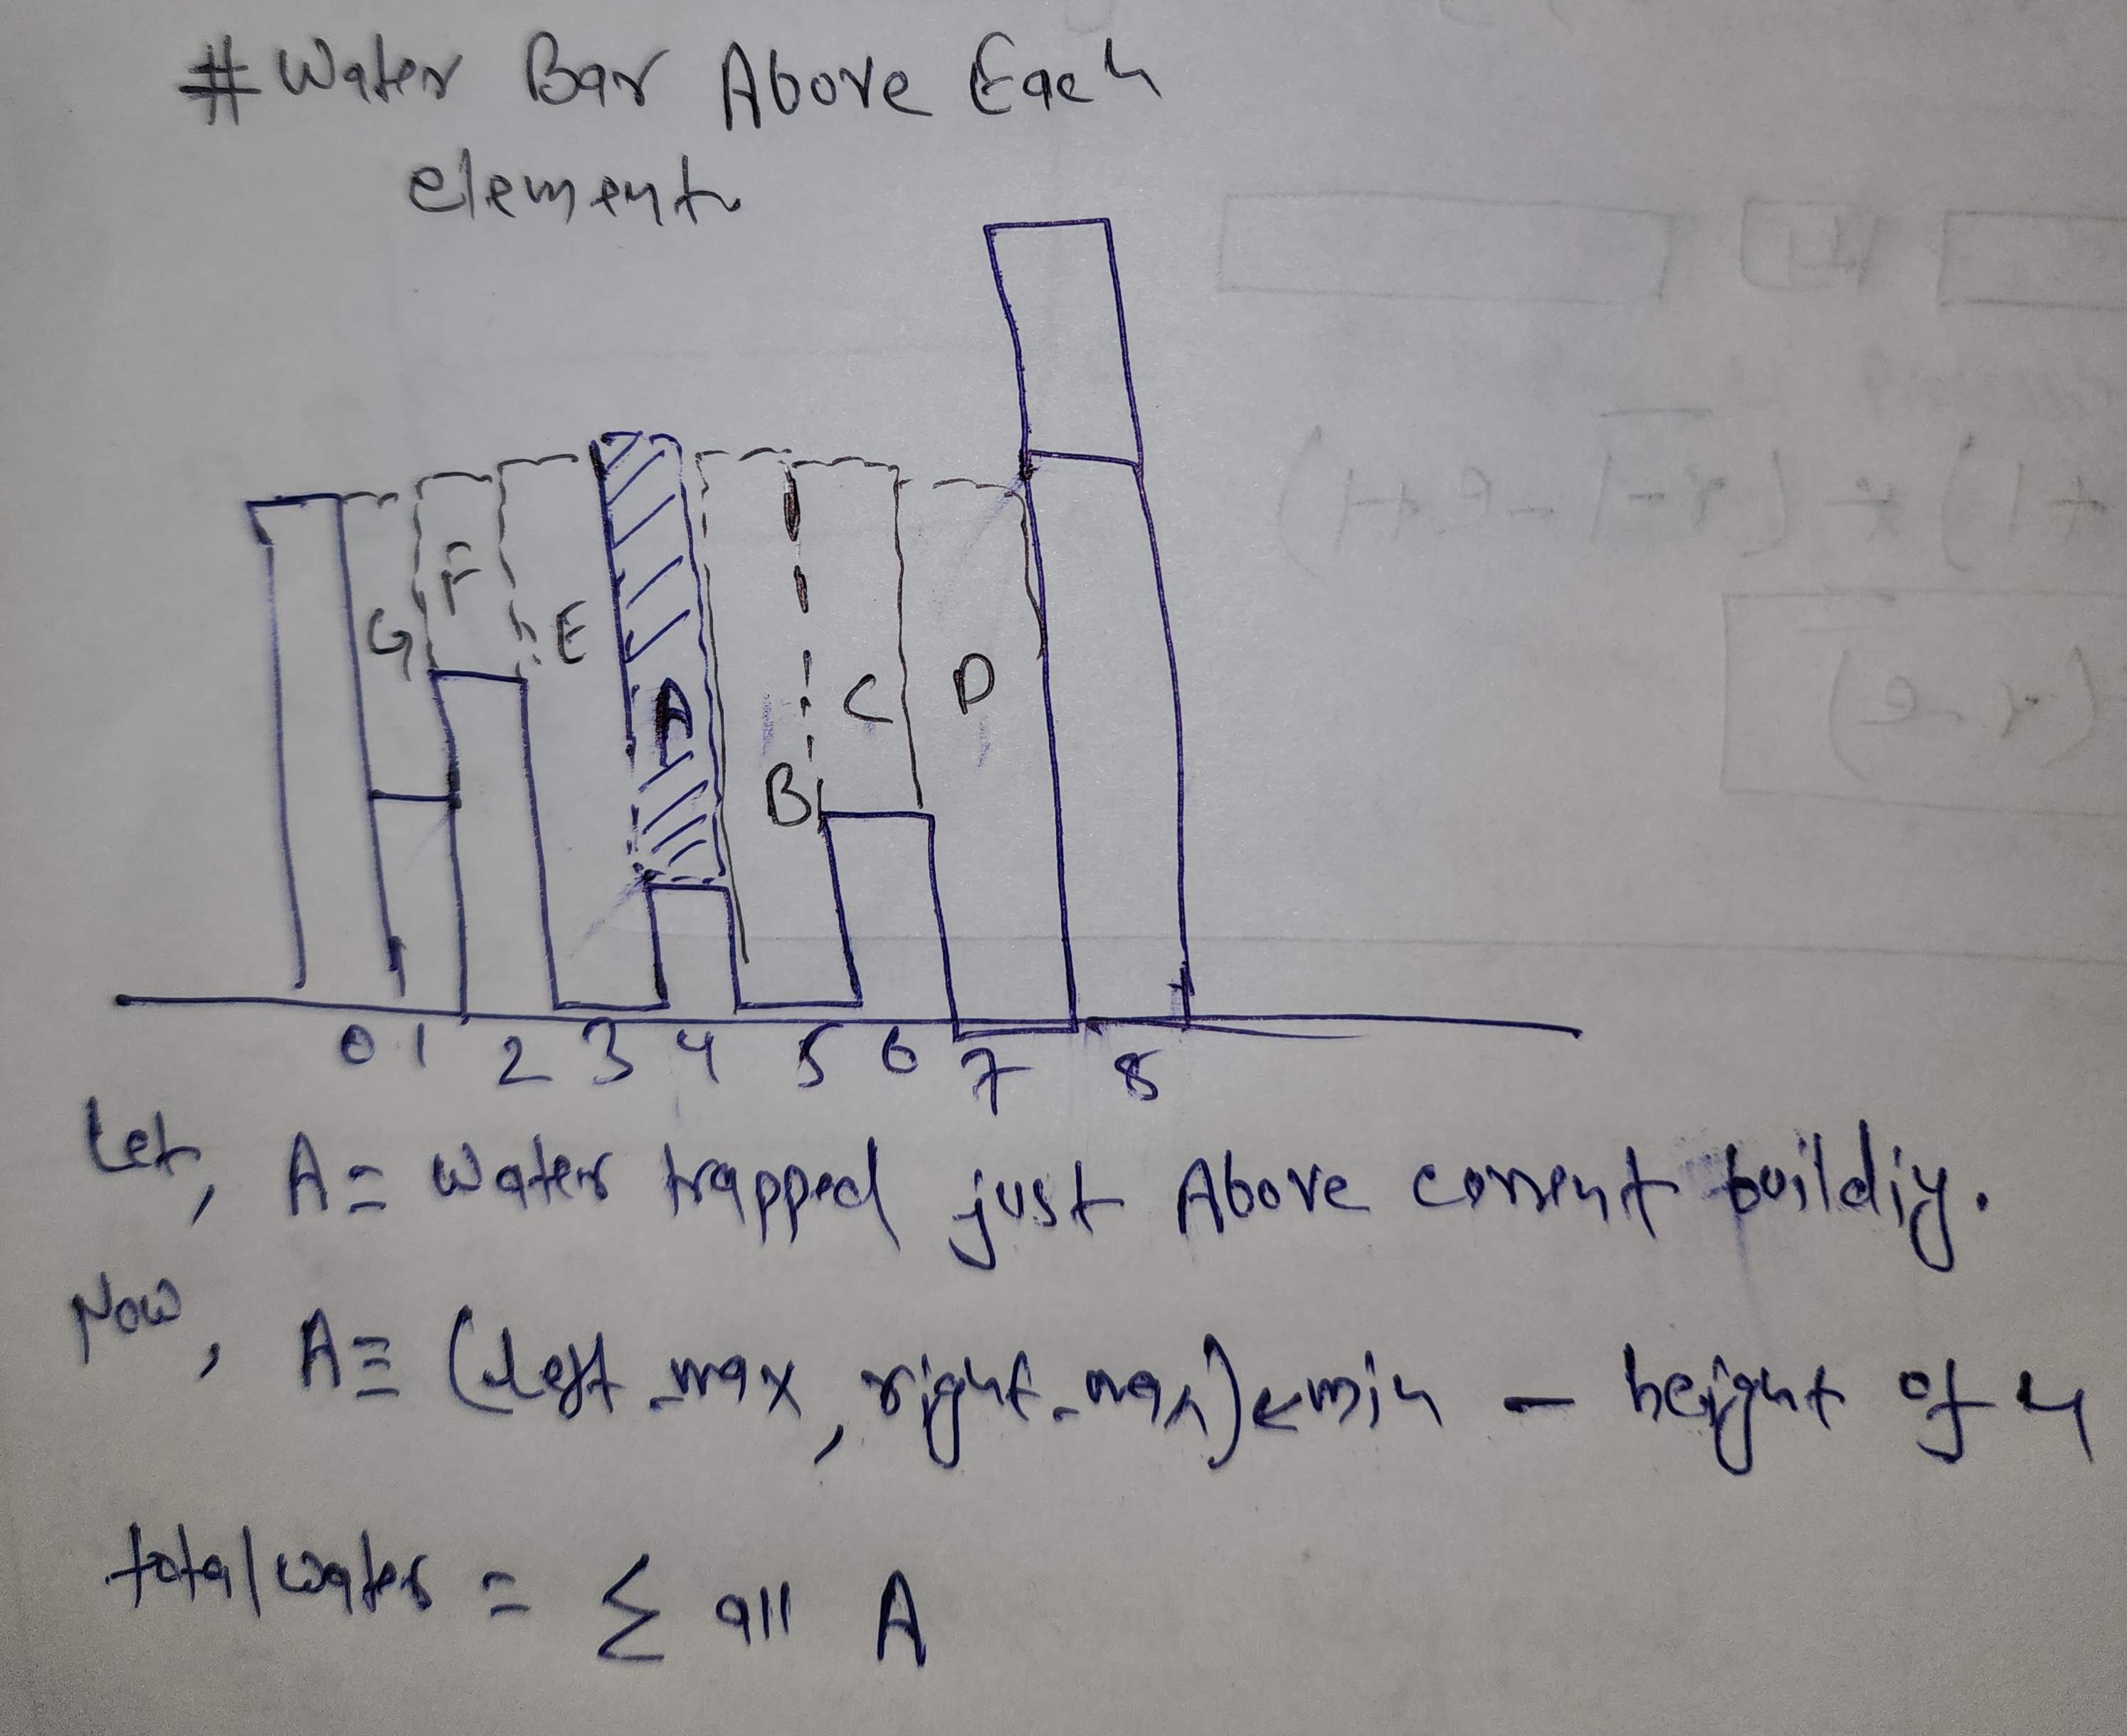
\includegraphics[width=\marginparwidth]{resources/stack-rain-water-harverstin-2.jpg}
    \end{marginfigure}
\end{solution}
    
\begin{solution}[Two Pointer | $O(1) space$]
    
    \begin{code}
//time: O(n)
//space: O(1) 
//BETTER
int twoPointerLogical(vector<int> height)
{
    int size = height.size();
    int left = 0,right = size-1;
    int leftMax = 0,rightMax = 0;
    
    int totalWater = 0;
    
    while(left < right)
    {
        if(leftMax < height[left] ) leftMax = height[left];
        if(height[right] > rightMax) rightMax = height[right];
        
        if(leftMax < rightMax)
        {
            totalWater += max(0,leftMax - height[left]);
            left++;
        }
        else
        {
            totalWater += max(0,rightMax - height[right]);
            right--;
        }
    }
    
    return totalWater; 
}
    \end{code}
\end{solution}